
% - - - - - - - - - - - - - - - - - - - - - - - - - - - - - - - - - - - - - - -

\begin{frame}{Cheap Talk Equilibrium - When Interests Align}
  Suppose that I want to meet up with Jose at a coffee shop on campus.
  \begin{table}[!h]
    \centering
    \begin{tabular}{cc|c|c|}
    & \multicolumn{1}{c}{} & \multicolumn{2}{c}{Jose}\\
    & \multicolumn{1}{c}{} & \multicolumn{1}{c}{$Starbucks$}  & \multicolumn{1}{c}{$Roma$} \\\cline{3-4}
    \multirow{2}*{Dante}  & $Starbucks$ & $1, 1$ & $0,0$ \\\cline{3-4}
                          & $Roma$       & $0, 0$ & $2,2$ \\\cline{3-4}
  \end{tabular}
  \end{table}

  We'll also add a first stage to this game 
  where Dante can send Jose a text message saying either 
  \textit{"I'm going to Starbucks"} or \textit{"I'm going to Roma"}.
\end{frame}

% - - - - - - - - - - - - - - - - - - - - - - - - - - - - - - - - - - - - - - -

\begin{frame}{Cheap Talk Equilibria - When Interests Align}
  The strategy profile where:
  \begin{itemize}
    \item  
    I send the message \textit{"going to Starbucks"}
    \item
    we both go to Starbucks if I send \textit{"going to Starbucks"}
    \item 
    or both go to Roma if I send \textit{"going to Roma"}
  \end{itemize}
  is a \textbf{Nash Equilibrium} (specifically a \textit{subgame perfect} NE).
  \begin{itemize}
    \item We'll call this a \alert{"cheap talk"} equilibrium 
    because it was in my best interest to communicate my actual strategy.
    \item It cost me nothing to send a \textit{message}.
  \end{itemize}
\end{frame}

% - - - - - - - - - - - - - - - - - - - - - - - - - - - - - - - - - - - - - - -

\begin{frame}{Cheap Talk vs Babbling Equilibrium}
  However, this is not the only SPNE of this game.
  If are strategy profiles in the second stage are:
  \begin{itemize}
    \item 
    Jose will go to Starbucks no matter what message Dante sends
    \item
    Dante will go to Starbucks no matter what message he sent
  \end{itemize}
  Then Dante will be indifferent between sending either message in the first place.

  \begin{itemize}
    \item 
    We'll call this a \alert{"babbling" equilibrium} 
    because the initial message sends \textit{no} information about what 
    I will actually do.
    \item 
    This equilibrium seems unlikely, but if I have an existing \textit{reputation}
    for always going to Starbucks, this would be plausible 
    and completely rational behavior.
  \end{itemize}
\end{frame}

% - - - - - - - - - - - - - - - - - - - - - - - - - - - - - - - - - - - - - - -

\begin{frame}{Cheap Talk Equilibria - When Interests are Conflicting}
  What about a zero-sum game?
  \begin{table}[!h]
    \centering
    \begin{tabular}{cc|c|c|}
    & \multicolumn{1}{c}{} & \multicolumn{2}{c}{Navratilova}\\
    & \multicolumn{1}{c}{} & \multicolumn{1}{c}{$DL$}  & \multicolumn{1}{c}{$CC$} \\\cline{3-4}
    \multirow{2}*{Evert}  & $DL$ & $50, 50$ & $80,20$ \\\cline{3-4}
                          & $CC$ & $90, 10$ & $20,80$ \\\cline{3-4}
  \end{tabular}
  \end{table}
  \begin{itemize}
    \item  
    Should Navratilova believe what Evert says she will do?
    \item 
    Should Navratilova believe that Evert will do 
    \textit{exactly the opposite} of what she says she'll do?
  \end{itemize}
\end{frame}

% - - - - - - - - - - - - - - - - - - - - - - - - - - - - - - - - - - - - - - -

\begin{frame}{Cheap Talk Equilibria - When Interests are Conflicting}
  What about a zero-sum game?
  \begin{table}[!h]
    \centering
    \begin{tabular}{cc|c|c|}
    & \multicolumn{1}{c}{} & \multicolumn{2}{c}{Navratilova}\\
    & \multicolumn{1}{c}{} & \multicolumn{1}{c}{$DL$}  & \multicolumn{1}{c}{$CC$} \\\cline{3-4}
    \multirow{2}*{Evert}  & $DL$ & $50, 50$ & $80,20$ \\\cline{3-4}
                          & $CC$ & $90, 10$ & $20,80$ \\\cline{3-4}
  \end{tabular}
  \end{table}
  \begin{itemize}
    \item 
    The only equilibrium of this game is a \alert{babbling} equilibrium.
    \item 
    There is no message that Evert could send
    that would give Navratilova any more idea of what she will actually play.
  \end{itemize}
\end{frame}

% - - - - - - - - - - - - - - - - - - - - - - - - - - - - - - - - - - - - - - -

\begin{frame}{Cheap Talk Equilibria - Partially Aligned Interests}
  Many real life games have mixtures of conflict and common interest.
  \begin{itemize}
    \item 
    The question of whether direct communication is \textit{credible} or not 
    will depend on the relative degree of each incentive.
    \item 
    We will use our tools from the first half of the course 
    to make testable predictions based on different ranges of assumptions.
  \end{itemize}
\end{frame}

% - - - - - - - - - - - - - - - - - - - - - - - - - - - - - - - - - - - - - - -

\begin{frame}{Defensive Medicine}
  \begin{quote}
    In a recent survey of physicians,
    93\% reported altering their clinical behavior 
    because of the threat of malpractice liability.
    Of them, 92\% used “assurance behavior” 
    such as ordering tests, performing diagnostic procedures,
    and referring patients for consultation;
    and 43\% reported using imaging technology 
    in clinically unnecessary circumstances. 
  \end{quote}  
  Harrington, pg. 461
\end{frame}

% - - - - - - - - - - - - - - - - - - - - - - - - - - - - - - - - - - - - - - -

\begin{frame}{Defensive Medicine}
  \begin{itemize}
    \item 
    Consider a patient who goes to the doctor for an examination. 
    \item
    The doctor can recommend an expensive test
    that is not fully covered by the patient's insurance.
    \item 
    The doctor cares about the patient, 
    but also doesn't want to be sued for malpractice 
    if the patient \textit{does} end up needing the test 
    and the doctor didn't recommend it.
    \item 
    The patients value $v$ from a beneficial test is 5,
    and $v=-5$ if the test is useless.
    \item 
    We'll use $a$ to stand in for the value of a test to a doctor 
    from a malpractice standpoint.
  \end{itemize}
\end{frame}

% - - - - - - - - - - - - - - - - - - - - - - - - - - - - - - - - - - - - - - -

\begin{frame}{Defensive Medicine}
  \begin{center}
    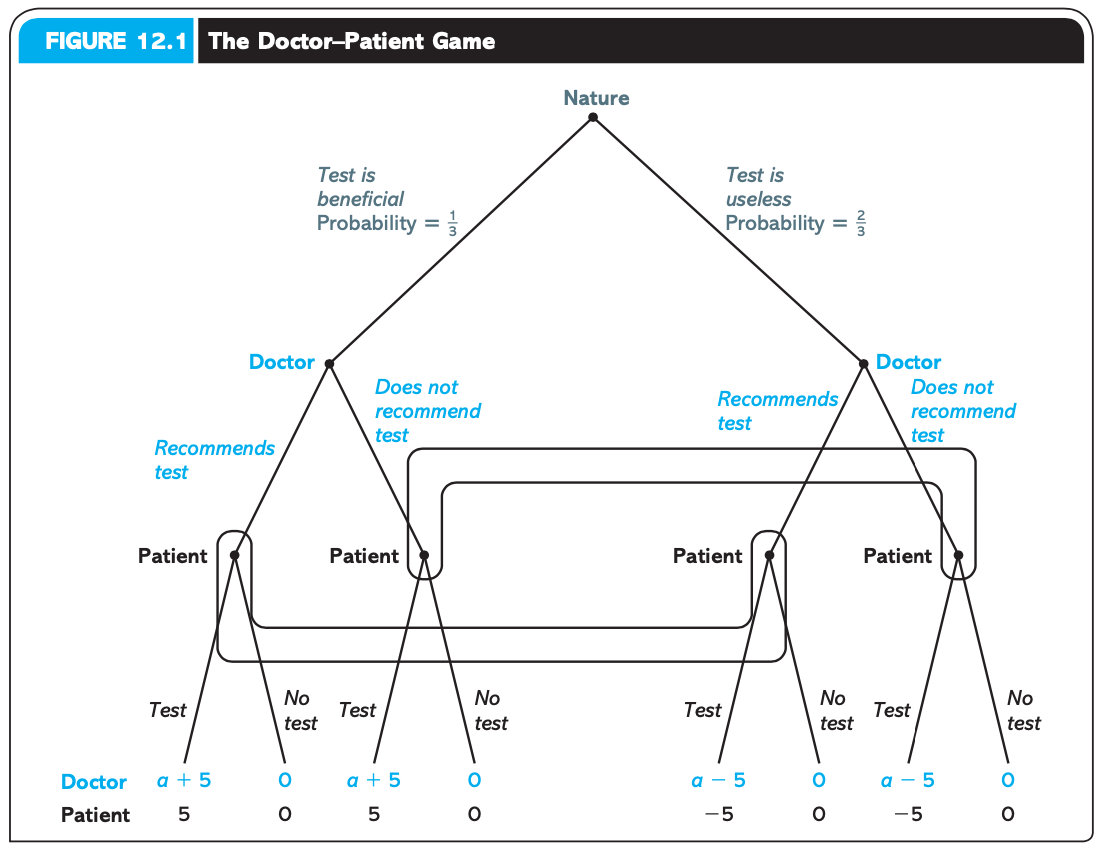
\includegraphics[width=.9\textwidth]{figures/defensivemed.png}  
  \end{center} 
\end{frame}

% - - - - - - - - - - - - - - - - - - - - - - - - - - - - - - - - - - - - - - -

\begin{frame}{Defensive Medicine - Babbling Strategy}
  % Why is defensive medicine so pervasive?
  \begin{block}{Pooling Equilibrium}
    \begin{itemize}
      \item \underline{Doctor's Strategy:}
      Recommend the test whether or not it is beneficial.
      \item \underline{Patient's Strategy:}
      Ignore the doctor's recommendation.
      \item \underline{Patient's Beliefs:}
      Ignoring the doctors advice,
      the probability the test is effective is 1/3.
    \end{itemize} 
  \end{block}
  \begin{itemize}
    \item This equilibrium is a \textit{babbling equilibrium}.
    \item The doctor's recommendation contains no real signal to the patient.
  \end{itemize}
\end{frame}

% - - - - - - - - - - - - - - - - - - - - - - - - - - - - - - - - - - - - - - -

\begin{frame}{Defensive Medicine - Babbling Strategy}
  % Why is defensive medicine so pervasive?
  \begin{block}{Pooling Equilibrium}
    \begin{itemize}
      \item \underline{Doctor's Strategy:}
      Recommend the test whether or not it is beneficial.
      \item \underline{Patient's Strategy:}
      Ignore the doctor's recommendation.
      \item \underline{Patient's Beliefs:}
      Ignoring the doctors advice,
      the probability the test is effective is 1/3.
    \end{itemize} 
  \end{block}
  \begin{itemize}
    \item The patient's beliefs are consistent, 
    and their expected utility from taking the test
    is $\frac{1}{3} \cdot 5 + \frac{2}{3} \cdot (-5) = - \frac{5}{3}$.
    \item Given that the patient will never take the test, 
    the doctor is indifferent between recommending the test or not.
    \item So this situation in which the doctor always recommends the test
    and the patient always ignores their advice is \textit{stable}.
  \end{itemize}
\end{frame}

% - - - - - - - - - - - - - - - - - - - - - - - - - - - - - - - - - - - - - - -

\begin{frame}{Defensive Medicine - Separating Strategies}
  The previous result was disappointing, but not unexpected.
  \begin{block}{Insight}
    For every cheap talk game, there is always a babbling equilibrium.
  \end{block}
  \begin{itemize}
    \item But let's now focus on the more interesting question
    of how to make the doctor's recommendation \textit{meaningful}.
  \end{itemize}
\end{frame}

% - - - - - - - - - - - - - - - - - - - - - - - - - - - - - - - - - - - - - - -

\begin{frame}{Defensive Medicine - Separating Strategies}
  Consider the following strategy profile:
  \begin{block}{}
    \begin{itemize}
      \item \underline{Doctor's Strategy:}
      Recommend the test if and only if it is beneficial.
      \item \underline{Patient's Strategy:}
      Follow the doctor's recommendation.
      \item \underline{Patient's Beliefs:}
      \begin{itemize}
        \item If the doctor recommends the test,
        then the test is beneficial with 100\% probability.
        \item If the doctor does not recommend the test,
        then the test is beneficial with 0\% probability.
      \end{itemize}
    \end{itemize}
  \end{block}
\end{frame}

% - - - - - - - - - - - - - - - - - - - - - - - - - - - - - - - - - - - - - - -

\begin{frame}{Defensive Medicine - Separating Strategies}
  When will the doctor follow the separating strategy?
  \begin{enumerate}
    \item When 
    $EU_d(\text{Rec. when beneficial}, (T,NT)) 
    \geq EU_d(\text{Don't rec. when beneficial}, (T,NT))$ 
    \vspace{12mm}
    \item and when 
    $EU_d(\text{Don't rec. when useless}, (T,NT)) 
    \geq EU_d(\text{Rec. when useless}, (T,NT))$ 
    \vspace{12mm}
  \end{enumerate}
  Solve for the range of $a$ where this is a NE.  
\end{frame}

% - - - - - - - - - - - - - - - - - - - - - - - - - - - - - - - - - - - - - - -


\begin{frame}{Defensive Medicine - Separating Strategies}
  When will the doctor follow the separating strategy?
  \begin{enumerate}
    \item When 
    $EU_d(\text{Rec. when beneficial}, (T,NT)) 
    \geq EU_d(\text{Don't rec. when beneficial}, (T,NT))$ 
    $$ a + 5 \geq 0 $$
    \item and when 
    $EU_d(\text{Don't rec. when useless}, (T,NT)) 
    \geq EU_d(\text{Rec. when useless}, (T,NT))$ 
    $$ 0 \geq a - 5 \Rightarrow a \leq 5 $$
  \end{enumerate}
  Solve for the range of $a$ where this is a NE.  
  $$  $$
\end{frame}

% - - - - - - - - - - - - - - - - - - - - - - - - - - - - - - - - - - - - - - -
\begin{frame}{Defensive Medicine - Conclusions}
  Interpreting our findings:
  \begin{itemize}
    \item 
    When $a=0$, the doctor's interests are \textit{perfectly} aligned 
    with the patient's.
    \item 
    When $a\leq5$, the doctor's interests are \textit{partially} aligned 
    with the patient's interests,
    and there is an equilibrium where the doctor gives truthful recommendations.
    \item 
    When $a>5$, there is only a babbling equilibrium
    because the doctor's incentives are to not be truthful.
    Even if they did give a truthful recommendation,
    the patient would have no reason to believe it would be \textit{credible}.
  \end{itemize}
\end{frame}

% - - - - - - - - - - - - - - - - - - - - - - - - - - - - - - - - - - - - - - -

\begin{frame}{Defensive Medicine - Conclusions}
  Connecting with our real-world observations:
  \begin{itemize}
    \item 
    We don't know what doctors' subjective costs of malpractice threats are
    ($a$).
    \item 
    But we can observe their \textit{behaviors}.
    \item 
    If we see that doctors recommend more tests than are beneficial,
    it might reveal that $a$ is quite large. 
  \end{itemize}
  \begin{block}{Revealed Preference}
    The idea that people reveal their true preferences by the choices they make.
  \end{block}
\end{frame}




